\documentclass{article}
\usepackage{tikz}
\usepackage{amsmath}
\usepackage[backend=biber,style=numeric,sorting=none]{biblatex}
\addbibresource{references.bib}


\title{Physics Workshop Notes}
\author{Workshop Instructor}

\begin{document}

\maketitle

\section{Introduction}

This workshop covers a basic physics concept.

\[
E = mc^{2}
\]
\[
-\frac{\hbar^{2}}{2m}\nabla^{2}\psi(\mathbf{r},t)+V(\mathbf{r})\,\psi(\mathbf{r},t)
= i\hbar\,\frac{\partial}{\partial t}\psi(\mathbf{r},t)
\]

This paper is super good! \cite{DrLimShuai}

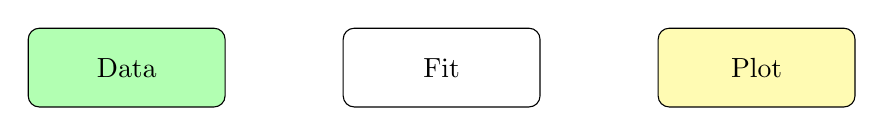
\begin{tikzpicture}
    \node[draw, fill=green!30, rounded corners, minimum width=2.5cm, minimum height=1cm] (data) at (0,0) {Data};
    \node[draw, fill=white, rounded corners, minimum width=2.5cm, minimum height=1cm] (fit) at (4,0) {Fit};
    \node[draw, fill=yellow!30, rounded corners, minimum width=2.5cm, minimum height=1cm] (plot) at (8,0) {Plot};
\end{tikzpicture}


\newpage
\printbibliography

\end{document}